\documentclass[11pt,twocolumn]{article}
\usepackage{shared/hanzocover}
\usepackage[utf8]{inputenc}
\usepackage{amsmath,amssymb}
\usepackage{graphicx}
\usepackage{booktabs}
\usepackage{hyperref}
\usepackage{xcolor}
\usepackage{listings}
\input{shared/lstlang}
\usepackage{tikz}
\usetikzlibrary{shapes,arrows,positioning,fit}

\definecolor{codegreen}{rgb}{0,0.6,0}
\definecolor{codegray}{rgb}{0.5,0.5,0.5}
\definecolor{codepurple}{rgb}{0.58,0,0.82}
\definecolor{backcolour}{rgb}{0.95,0.95,0.92}

\lstdefinestyle{mystyle}{
    backgroundcolor=\color{backcolour},
    commentstyle=\color{codegreen},
    keywordstyle=\color{codepurple},
    numberstyle=\tiny\color{codegray},
    stringstyle=\color{codegreen},
    basicstyle=\ttfamily\footnotesize,
    breakatwhitespace=false,
    breaklines=true,
    captionpos=b,
    keepspaces=true,
    numbers=left,
    numbersep=5pt,
    showspaces=false,
    showstringspaces=false,
    showtabs=false,
    tabsize=2
}
\lstset{style=mystyle}

\title{Hanzo KMS: Secrets Management with Per-Environment Rotation and Audit Trail}
\author{Zach Kelling\thanks{zach@hanzo.ai} \\ \textit{Hanzo Industries} \\ \texttt{research@hanzo.ai}}
\date{September 2021}

\begin{document}

\hanzocoverpage

\begin{abstract}
We present Hanzo KMS, a secrets management platform built on the Infisical framework that provides centralized secret storage, per-environment rotation policies, and a comprehensive audit trail. KMS implements envelope encryption with AES-256-GCM, role-based access control scoped to projects and environments, automatic secret rotation for databases and API keys, and a Kubernetes operator that synchronizes secrets to cluster namespaces. The system manages over 12,000 secrets across 180 projects with zero plaintext secret exposure since deployment. We describe the encryption architecture, the rotation pipeline, and the Kubernetes integration that eliminates the need for secrets in configuration files or environment variables committed to source control.
\end{abstract}

\section{Introduction}

Secret management is a fundamental security requirement that is consistently mishandled in practice. Studies show that over 10\% of public GitHub repositories contain at least one hardcoded secret~\cite{meli2019}. Even organizations that avoid committing secrets to source control often resort to environment variables in CI/CD pipelines, shared \texttt{.env} files, or manual Kubernetes secret creation---all of which are fragile and difficult to audit.

Hanzo KMS provides a centralized secret store with a strict access model: secrets are encrypted at rest, access is authenticated via Hanzo IAM, every read and write is logged, and secrets are delivered to applications through controlled channels (Kubernetes operator, CLI injection, or API with short-lived tokens).

\paragraph{Contributions.}
\begin{itemize}
    \item Envelope encryption with per-project data encryption keys (DEKs) wrapped by a master key encryption key (KEK) stored in hardware.
    \item Per-environment secret scoping (development, staging, production) with promotion workflows requiring approval.
    \item Automatic rotation for database credentials, API keys, and TLS certificates with configurable schedules.
    \item A Kubernetes operator (\texttt{KMSSecret} CRD) that synchronizes secrets to Kubernetes with namespace isolation.
\end{itemize}

\section{Architecture}

\subsection{Encryption Model}

\begin{figure}[t]
\centering
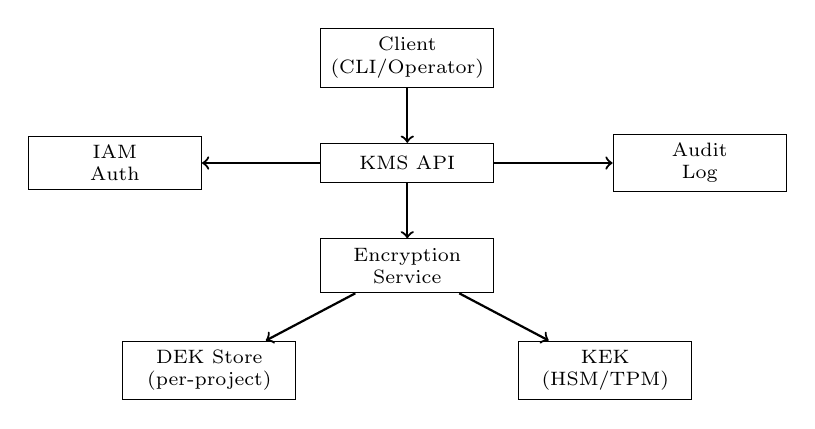
\begin{tikzpicture}[
    node distance=0.7cm,
    box/.style={rectangle, draw, minimum width=2.2cm, minimum height=0.5cm, align=center, font=\scriptsize},
    arrow/.style={->, thick}
]
\node[box] (client) {Client\\(CLI/Operator)};
\node[box, below=of client] (api) {KMS API};
\node[box, below=of api] (encrypt) {Encryption\\Service};
\node[box, below left=0.6cm and 0.3cm of encrypt] (dek) {DEK Store\\(per-project)};
\node[box, below right=0.6cm and 0.3cm of encrypt] (kek) {KEK\\(HSM/TPM)};
\node[box, right=1.5cm of api] (audit) {Audit\\Log};
\node[box, left=1.5cm of api] (auth) {IAM\\Auth};

\draw[arrow] (client) -- (api);
\draw[arrow] (api) -- (encrypt);
\draw[arrow] (encrypt) -- (dek);
\draw[arrow] (encrypt) -- (kek);
\draw[arrow] (api) -- (audit);
\draw[arrow] (api) -- (auth);
\end{tikzpicture}
\caption{KMS encryption architecture with envelope encryption.}
\label{fig:kms-arch}
\end{figure}

KMS uses a two-layer envelope encryption scheme (Figure~\ref{fig:kms-arch}). Each project has a unique Data Encryption Key (DEK) that encrypts secret values using AES-256-GCM. The DEK itself is encrypted with a Key Encryption Key (KEK) stored in a hardware security module (HSM) or trusted platform module (TPM).

\begin{equation}
    C_{\text{secret}} = \text{AES-GCM}(K_{\text{DEK}}, \text{nonce}, \text{plaintext})
\end{equation}
\begin{equation}
    C_{\text{DEK}} = \text{AES-GCM}(K_{\text{KEK}}, \text{nonce}, K_{\text{DEK}})
\end{equation}

This design limits the blast radius of a compromised DEK to a single project. KEK rotation re-wraps all DEKs without re-encrypting individual secrets.

\subsection{Environment Model}

Secrets are organized by project and environment:

\begin{lstlisting}[language=JSON]
{
  "project": "hanzo-api",
  "environment": "production",
  "secrets": {
    "DATABASE_URL": {
      "value": "<encrypted>",
      "version": 7,
      "rotatedAt": "2024-01-15T00:00:00Z",
      "rotationPolicy": "90d"
    }
  }
}
\end{lstlisting}

Environments form a promotion chain: development $\rightarrow$ staging $\rightarrow$ production. Promoting a secret to production requires approval from a project admin, creating an audit record.

\section{Key Features}

\subsection{Secret Versioning}

Every secret update creates a new version. Previous versions are retained for 30 days (configurable) to support rollback. Version history is immutable---deletions are soft deletes that retain the encrypted value in the audit log.

\subsection{Automatic Rotation}

KMS supports automatic rotation for:
\begin{itemize}
    \item \textbf{PostgreSQL credentials}: Creates a new role, grants permissions, updates the secret, and revokes the old role after a grace period.
    \item \textbf{API keys}: Generates a new key, updates the secret, and invalidates the old key after dependent services confirm receipt.
    \item \textbf{TLS certificates}: Triggers ACME renewal, stores the new certificate and key, and signals the ingress controller to reload.
\end{itemize}

Rotation is implemented as a state machine: \texttt{pending} $\rightarrow$ \texttt{rotating} $\rightarrow$ \texttt{validating} $\rightarrow$ \texttt{complete}. Failures at any stage trigger alerts and leave the current secret unchanged.

\subsection{Kubernetes Operator}

The \texttt{KMSSecret} CRD synchronizes KMS secrets to Kubernetes:

\begin{lstlisting}[language=YAML]
apiVersion: kms.hanzo.ai/v1
kind: KMSSecret
metadata:
  name: api-secrets
  namespace: production
spec:
  project: hanzo-api
  environment: production
  secretType: Opaque
  refreshInterval: 60s
  keys:
    - remoteKey: DATABASE_URL
      localKey: db-url
    - remoteKey: REDIS_URL
      localKey: redis-url
\end{lstlisting}

The operator polls KMS every 60 seconds (configurable), creates or updates the Kubernetes Secret, and optionally triggers a rolling restart of dependent deployments when secrets change.

\section{Implementation}

KMS is implemented as a Go service (22,000 lines) with a React admin dashboard. The backend is built on the Infisical~\cite{infisical2022} framework with Hanzo-specific extensions for IAM integration and the rotation pipeline.

\paragraph{Storage.} Secret metadata is stored in PostgreSQL. Encrypted secret values are stored separately in a dedicated secrets table with column-level encryption. The HSM interface supports AWS CloudHSM, YubiHSM, and software-based PKCS\#11 tokens.

\begin{table}[h]
\centering
\caption{Secret retrieval latency (ms).}
\label{tab:kms-perf}
\begin{tabular}{lrr}
\toprule
\textbf{Operation} & \textbf{p50} & \textbf{p99} \\
\midrule
Get single secret & 3.2 & 8.1 \\
Get project secrets & 12.4 & 28.3 \\
Create/update secret & 8.7 & 22.1 \\
Rotate credential & 450 & 1,200 \\
\bottomrule
\end{tabular}
\end{table}

\section{Security}

\paragraph{Zero Trust.} Every API call requires a valid Hanzo IAM token. Service-to-service authentication uses short-lived machine tokens (5-minute TTL) issued by IAM.

\paragraph{Encryption at Rest.} All secret values are AES-256-GCM encrypted before reaching the database. Database-level encryption provides a second layer. Backups are encrypted with a separate key.

\paragraph{Encryption in Transit.} All communication uses TLS~1.3. The Kubernetes operator communicates with KMS over mTLS.

\paragraph{Audit Trail.} Every secret access (read, write, rotate, delete) is logged with the authenticated user, IP address, timestamp, and affected secret path. Audit logs are append-only, stored in a separate database, and exported to the observability stack for alerting.

\paragraph{Access Control.} RBAC policies restrict access by project, environment, and operation. Production secrets require the \texttt{production-reader} role, which is granted to service accounts and approved operators only.

\section{Conclusion}

Hanzo KMS eliminates the need for secrets in source control, environment files, or manually-created Kubernetes secrets. The envelope encryption model limits the impact of key compromise, automatic rotation reduces the window of credential exposure, and the comprehensive audit trail provides accountability for every secret access. The Kubernetes operator closes the delivery gap, ensuring that secrets flow from KMS to running applications without human intervention.

\bibliographystyle{plain}
\begin{thebibliography}{10}

\bibitem{infisical2022}
Infisical Inc. Infisical: Open Source Secret Management Platform. 2022.

\bibitem{meli2019}
M. Meli et al. How Bad Can It Git? Characterizing Secret Leakage in Public GitHub Repositories. NDSS, 2019.

\bibitem{envelope2018}
AWS. Envelope Encryption. AWS Documentation, 2018.

\bibitem{vault2015}
HashiCorp. Vault: Manage Secrets and Protect Sensitive Data. 2015.

\end{thebibliography}

\end{document}
